\documentclass{article}
\usepackage[utf8]{inputenc}
\title{Lecture 6: probabilistic models}
\author{wbg231 }
\date{December 2022}
\newcommand{\R}{$\mathbb{R}$}
\newcommand{\B}{$\beta$}
\newcommand{\A}{$\alpha$}
\newcommand{\D}{\Delta}

\newcommand{\avector}[2]{(#1_2,\ldots,#1_{#2})}
\newcommand{\makedef}[2]{$\textbf{#1}$:#2 }
\usepackage{tikz,graphicx,hyperref,amsmath,amsfonts,amscd,amssymb,bm,cite,epsfig,epsf,url}

\begin{document}

\maketitle

\section{overview}
\begin{itemize}
\subsection{why probabilistic models}
\item gives us a unified framework for many models 
\item allows us to take tools form probability theory and use them to solve problems 
\itme it also gives us a principled way to insert previous info into our model 
\subsection{today's lecture}
\item there are two ways to model data generation. \item 1. conditional $P(y|x)$
\item generative models we want to learn the joint $P(x,y)$ and use that to make predictions 
\item we want to understand how can we build these models and estimate there parameters 
\item in both cases we use mle 
\item and we can compare generative and conditional models 
\section{conditional models}
\subsection{linear regression}
\item lets start with an example
\item our goal is to predicted $y\in \mathbb{R}$ using our feature vector $x$ from our data. 
\item could be house pricing, medical prediction, age of person based on photo etc
\subsection{problem set up}
\item data training examples $D=\{(x_i,y_i)\}_{i=1}^{n}$ where $x\in \mathbb{R}^d$ and $y\in\mathbb{R}$
\item model: a linear function$ h$ with parameter $\theta$ to predict y from x $$h(x)=\Sigma_{i=1}^{d}\theta_ix_i=\theta^tx$$ where $\theta\in\mathbb{R}^d$ are our weights
\itme we predict the label as a linear function of our inputs 
\item we Incorporated a bias term (also called interpret) into x
\subsection{parameter estimation}
\item loss function:we estimate  $\theta$ by minimizing the square loss (the least squared method)$$j(\theta)=\frac{1}{n}\Sigma_{i=1}^{n}(y^i-\theta^tx^i)^2$$ (empirical risk)
\item let $X\in \mathbb{R}^{n\timed d}$
 be the design matrix whose rows are input features 
 \item let $y\in \mathbb{R}^{n}$ by the vector of all targets 
 \item we want to find $$\hat{\theta}=agmin_{\theta}J(\theta)=argmin_{\theta}(X\theta-y)^t(X\theta-y)$$
 \item we can see that $\nabla j(\theta)= 2X^tX\theta-2X^Ty$ which yields
 \item closed form solution $\hat{\theta}=(X^TX)^{-1}X^ty$
 \item note here that $(X^TX)\in \mathbb{R}^{d\times d}$ may not be invertable. 
 \item recall that for a matrix $A\in \mathbb{R}^{n\times d}, rank(A)$ is the minimum number of linearly independent rows and columns in that matrix, and further $rank(A^T)=rank(A)$ and for any two matrices $rank(AB)\leq min(rank(a),rank(b))$
 \item so in this case $rank(A^TA)\leq min(rank(a),rank(a^T))\leq min(n,d)$
 \item so in other words we must have at least d linearly independent examples, as well as all linearly independent features for our closed form solution to exist and be unique.
 \item we know that $X^TX$ is positive semi-definite so if it not invertable then there is a null space, meaning we can add any vector in the null space to our solution and thus the solution is not unique. 
 \subsection{review}
 \item so far we have seen linear regression, we assume that there is a linear function of our input and we take the best model based on the square loss.
 \item but why do we use the square loss? 
 \item what are the assumptions we are making about our model and data that bring us to the square loss
 \item how can we look at it from a different perspective, and what do we need to assume about our data in terms of probability to derive this objective? 
 \subsection{assumptions in linear regression}
\item how can we derive the objective form the data 
\item we assume that there is a linear function with some noise $(\epsilon)$ mapping x to y. that is $$y=\theta^tx+\epsilon$$
\item where we call $\epsilon$ the residual error capture all unmodeld effects eg noise
\item further we assume t=hat the errors are distributed iid according to $$\epsilon\sim \mahtcal{N}(0,\sigma^2)$$
 \item so what is the conditional distribution  $Y|X=x$ (here capitals are rv)
 \begin{itemize}
     \item well we know $Y|x=x$ is given by $y=\theta^tx+\epsilon$
     \item where $x$ and $\theta$ are fixed 
     \item thus $E[y]=E[\theta^tx+\epsilon]=E[\theta^tx]+E[\epsilon]=E[\theta^tx]+0=\theta^tx$
     \item and variance is $var(y)=var(\theta^Tx+\epsilon)=var(\theta^tx)+var(\epsilon)+2cov(\theta^tx,y)=0+\sigma^2+0=\sigma^2$
     \item thus $Y|X=x\sim \mathcal{N}(\theta^tx,\sigma^2)$
 \end{itemize}
 \item so in other words we are assuming that $Y|X=x$ is just a normal Gaussian shifted. this can be thought of as putting a Gaussian bump around the output of the linear predictor. 
 \item so this is a linear map with some Gaussian noise around the results. 
 \item this is an assumption this may be true, it may be untrue. 
 \subsection{Maximum likelihood estimator}
 \item so given a probabilistic model and dataset $\mathcal{D}$ how do we estimate $\theta$? Assuming that our examples are iid
 \item the maximum likelihood principle stats that we should max the conditional likelihood of our data that is $$\mathcal{L}(\theta)=P(\mathcal{D}|\theta)=P(y_1...y_n|\theta x_1...\theta x_n)=\Pi_{i=1}^{n}P(y^i|x^i,\theta)$$
 \item in practice we use the log log likelihood since it makes is easier to work with really small values, and sometimes try to minimize the negative log likelihood. 
 \subsection{mle for linear regression}
 \item so we can write $\\\ell(\theta)=\\\log(\mahtcal{L}(\theta)=\\log\Pi_{i=1}^{n}P(y^i|x^i,\theta)\\\Sigma_{i=1}^{n}log(p(y^i|x_i,\theta))=\\\Sigma_{i=1}^{n}log(\frac{1}{\sqrt{w\pi}\sigma}e^{-\frac{1}{2}(\frac{y^i-\theta^tx_i}{\sigma})^2} )=\\
 \Sigma_{i=1}^{n}log(\frac{1}{\sqrt{w\pi}\sigma}e^{-(\frac{(y^i-\theta^tx^i)^2} {2(\sigma)^2}} )\\
 =
 \Sigma_{i=1}^{n}(log(\frac{1}{\sqrt{w\pi}\sigma})-\frac{(y^i-\theta^tx^i)^2} {2(\sigma)^2})=\\ 
 n(log(\frac{1}{\sqrt{w\pi}\sigma})-\frac{1}{2\sigma^2}\Sigma_{i=1}^{n}(y^i-\theta^tx^i)^2
 $
 \item our goal is to maximise this function,so we can take the gradient 
\item so first off note that we can write $$\ell(\theta)= n(log(\frac{1}{\sqrt{w\pi}\sigma})-\frac{1}{2\sigma^2}\Sigma_{i=1}^{n}(y^i-\theta^tx^i)^2= n(log(\frac{1}{\sqrt{w\pi}\sigma})-\frac{1}{2\sigma^2}\Sigma_{i=1}^{n}(y^i)^2-2\theta^tx^iy^i+(\theta^tx^i)^t(\theta^tx^i)$$
\item then we can see that $\frac{\partial \ell}{\partial \theta_i}=-\frac{1}{2\sigma^2}\Sigma_{j=1}^{n}(2y^jx^j_i-2\theta x^jx^j_i)=-\frac{1}{\sigma^2}\Sigma_{j=1}^{n}(y^j-\theta x^j)x^j_i$
\item than we can set that two zero and see that $\theta^*=\Sigma_{j=1}^n\frac{y^jx_i^j}{x^jx^j_i}$
\item then if we take the derivative with rep sect to $\theta$ as a vector we get $\theta^*=\Sigma_{i=1}^{n}\frac{x^iy^y}{(x^i)^t x_i}=(X^TX)^{-1}(X^Ty)$ which is the linear regression solution 
\subsection{review}
\item so if we assume that our data generating process is Gaussian it is the same as doing least squares. 
\item but what if our data is not Gaussian
\section{logistic regression}
\item consider binary classification $y\in \{0,1\}$ that should the conditional distribution be? we model $P(Y|X=x)$ as a Bernoulli such that $$P(y|x)=h(x)^y(1-h(x))^{1-y}$$ 
\item how should be parameterize y?
\begin{itemize}
    \item what is $P(y=1|x)$ and $P(y=p|x_$ where $h(x)\in (0,1)$? these are basically transformed linear regressions models
    \item what is the mean $Y|X=x$?
    \tme we need a function f to map the linear predictor $\theta^tx\in \mathbb{R}$ to (0,1)? $E[Y|X=x]=\Sigma_{y\in y}yP(y=y|x=x)=1P(y=1|x=x)+0P(y=0|x=x)=P(y=1|x=x)$
    \item we define the logistic function as $$f(\eta)=\frac{1}{1+e^-\eta}$$
\end{itemize}
\item the logistic function looks like this \\ 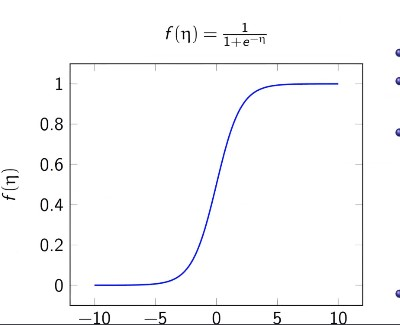
\includegraphics[width=10cm]{lecture_notes/lecture_6/immages/lecture_6_1.jpg}
\item  $P(y|x)=$Bernoulli$f(\theta^tx)$
\begin{itemize}
    \item look at the log odds $log(\frac{P(y=1|x)}{P(y=0|x)})=\theta^Tx$ 
    \item this can be expressed as $log(P(y=1|x))-log(p(y=0|x)$
    \item recall that we can write $P(y|x)=P(y|x)=h(x)^y(1-h(x))^{1-y}$ 
    \item so thus we have $ log(\frac{P(y=1|x)}{P(y=0|x)})=\theta^Tx=log(P(y=1|x))-log(p(y=0|x)=log(f(x)^1(1-h(x))^{1-1})-log(f(x)^(0)(1-h(x))^{1-0})=log(f(x))-log(1-f(x))=log(\frac{1}{1+e^{-\eta}})-log(1-\frac{1}{1+e^{-\eta}})=log(1)-log(1+e^{-\eta})-log(\frac{1+\eta^-n-1}{1+\eta^-n}=log(1+e^{-\eta})-log(\frac{e^-\eta}{1+e^{-\eta}}=log(1+e^{-\eta})-log(e^{-\eta})+log(1+e^{-\eta})=-log(e^{-\eta})=\eta=\theta^tx$
    \item so in other words the log odds are a linear function that form a decision boundary, that is a linear decision boundary
    \item this means the decision boundary is linear, ie the features are linear in the parameter as we increase the value of $\theta^tx$ we get 1, and as we decrees it we get zero
\end{itemize}
\item how can we extend this to multi-class classification?
\subsection{mle for logistic regression}
\item we would again like to max our conditional log likely hood
\item $\ell(\theta)=log(\mathcal{L}(\theta))=\Sigma_{i=1}^{n}log (P(y^i|x^i,\theta))=\Sigma_{i=1}^{n}log((f(\theta^t x^i)^y^i(1-f(\theta^t x^i))^{1-y^i})=\Sigma_{i=1}^{n}y^ilog(f(\theta^t x^i)+({1-y^i})log(1-f(\theta^t x^i))$
\item this does not have a closed form solution, but the likelihood is concave so we can use gradient ascent to get a unique optimal solution 
\subsection{gradient ascent for logistic regression}
\item so call gradient ascent $\theta=\theta+\nabla \ell(\theta)$
\item so call the liklyhood of a single example $\ell_n=r^nlog(f(\theta^tx^n)+(1-y^n)log(1-f(\theta^Tx^n))$
\item then we can see that $\frac{\partial \ell^n}{\partial \theta_i}=\frac{\partial \ell^n}{\partial f^n}\frac{\partial f^n}{\partial \theta_i}=(\frac{y^n}{f^n}-\frac{1-y^n}{1-f^n})\frac{\partial f^n}{\partial \theta_i}$
\item recall that $f^n(\theta^t x^i)=\frac{1}{1+e^{-\theta^t x_i}}$ 
\item thus we have $\frac{\partial f^n}{\theta_i}=\frac{\partial f^n}{e^{-\theta x_i}}\frac{\partial e^{-\theta x_i}}{\partial -\theta^tx_i}\frac{\theta^tx_i}{\theta_i}=\frac{-1}{(1+e^{-\theta^tx_i})^2}-e^{\theta^t x_i}x_i_j$
\item thus we have $\frac{\partial \ell^n}{\partial \theta_i}=\frac{\partial \ell^n}{\partial f^n}\frac{\partial f^n}{\partial \theta_i}=(\frac{y^n}{f^n}-\frac{1-y^n}{1-f^n})\frac{\partial f^n}{\partial \theta_i}=\frac{\partial \ell^n}{\partial f^n}\frac{\partial f^n}{\partial \theta_i}=(\frac{y^n}{f^n}-\frac{1-y^n}{1-f^n})(f^n(1-f^n)x_i^n)=(y^n-f^n)x_i^n$
\item and then if we take the full partial we get $\frac{\partial \ell}{\partial \theta_i}=\Sigma_{j=1}^{n}(y^j-f(\theta^tx^j))x^j_i$
\subsection{compare linear and logistic regression}
\item linear
\begin{itemize}
    \item it is linear 
    \item outputs real numbers
    \item we assume that conditional distribution $Y|X=x$ is Gaussian
    \item the transfer function $F(\theta^tx_i)$ is identity 
    \item and the mean $E[Y|X=x,\theta]=\theta^tx$ since we assumed that $Y|x=x\sim N(\theta^tx, \sigma^2)$
\end{itemize}
\item logistic
\begin{itemize}
    \item it is linear 
    \item outputs categorical variables
    \item we assume that condital distrobution $Y|X=x$ is bernuli 
    \item the transfer function  is logistic 
    \item is also $f(\theta^t x)$ (i think this has to do with the log likelihood being that. 
\end{itemize}
\item the main difference between the two how we model the conditional distribution
\section{generalized regression model}
\item suppose we have $x$ and we want to predict $P(y|x)$
\item for modeling we Can chose a parametric family of distributions $P(y,\theta)$ with parameters $\theta\in \Theta$
\item chose a transfer function that maps a linear predictor in $\mathbb{R}$ to $\Theta$ $$x\in \mathbb{R}^d\rightarrow (w^tx)\in \mathbb{R}\rightarrow f(w^tx)\in \Theta =\theta$$
\item so we can train this model using MLE $$\hat{\theta}\in argmax_{\theta}logp(\mathcal{D},\hat{\theta})$$ 
\item and make predictions as $x\rightarrow f(w^tx)$
\item so the transfer function in linear regression is identity
\item the transfer function in logistic regression is the logistic function
\item these algorithms only deffer based on the transfer function 
\item so the idea is we can do kind of simple regression, then use a transfer function to transom that model into the context we are working in (that is into our parametric family of distributions. ) 
\subsection{example Poisson regression}
\item say we want to predict the number of people enter a restaurant in NYC during lurch time 
\item what features can be use dull, what i a good model for the number of visitors
\item recall that a passion random variable $Y$ with parameter $\lambda$ has conditional $$P(y=k,\lambda)=\frac{\lambda^ke^{-\lambda}}{k!}$$ this is a good model for the number of events that occur with in a period of time 
\item so suppose we say that our conditional distribution $Y|X=x\sim$Poisson$(\lambda)$
\item x enters linearly that is $$x\rightarrow w^Tx\rightarrow \lambda=f(w^tx)$$ so that is we are using standard linear regression to learn a parameter $\lambda$ that we then use as the parameter in our Poisson model 
\item standard approach is to use the exponential distribution ie $f(w^tx)=exp(w^tx)$
\item the log likelihood of the full dataset $\mathcal{D}$ under our assumptions is 
$$log(p(\mathcal{D},\lambda _i)=\Sigma_{i=1}^{n}log(\frac{\lambda^{y_i}e{-\lambda}}{y_i!})=\Sigma_{i=1}^{n}[y_ilog(\lambda_i)-\lambda_i-log(y_i!)]=log(p,\mathcal{D},w)$$ $$=\Sigma_{i=1}^{n}[y_ilog(exp(w^tx_i))-exp(w^tx_i)-log(y_i!)]=\Sigma_{i=1}^{n}[y_iw^tx_i-exp(w^tx_i)-log(y_i!)]$$
\item we can take derivatives of this and try to solve it. 
\item this is an example of how we can model a problem by specifying our assumptions about the model. 
\subsection{multinomal logistic regression example}
\item we are going to extend the logistic regression to multiple classes
\item so we parameterize this with a probability vector $\theta\in \mathbb{R}^{k}$ where there are k classes.
\item a probability vector $\theta$ has the following properties
\begin{itemize}

\item $\sigma_{i=1}^{n}\theta_i=1$ and $\theta_i\geq 0$
\item and $\forall y\in [1,k] P(Y=y)=\theta_y$
\end{itemize}
\item for each x we compute a linear score function for each class that is $$x\rightarrow [<w_1,x>,,,<w_k,x>]\in \mahtbb{R}^d$$
\item and we use the soft max function as our transfer function 
$$(s_1..s_k)\rightarrow \theta = (\frac{e^{s_1}}{\Sigma_{i=1}^{n}e^{s_i}}...\frac{e^{s_k}}{\Sigma_{i=1}^{n}e^{s_i}})$$
\item it is kind of a way to normalize everything so the likelihood over all classes sum to one and all values are positive

\item how to predict class of a new entry $x\in\mathbb{R}^d$
\begin{itemize}
    \item first we compute the scores $x\rightarrow [<w_1,x>,,,<w_k,x>]\in \mahtbb{R}^d\rightarrow \theta$
    \item then we take the soft max of $\theta, f(\theta)$
    \item we can write the conditional probability for class y as $$P(y|x,w)=\frac{e(w^t_yx)}{\Sigma_{i=1}^{k}e^{w_i^tx}}$$
    \item so we would take the arg max over y as the final prediction 
\end{itemize}
\subsection{review}
\item we have so far seen how to construct a model, so that our problem can be solved in a more principled probabilistic point of view
\item the most important thing is to chose the output distribution bass ed on the input data, and takes that we have 
\item as well as the transfer function which maps a linear combination of the input to the parameter, then we cal learn it using mle and gradient descent 
\item this family of models are called generalized linear models 
\item the parameters of the function are linear , but the distribution themselves may not be linear. 
\section{generative models}
\subsection{review}
\item so far we have dealt with conditional models that is finding $P(y|x)$
\item now we want to find the joint of y,x that is $P(x,y,\theta)$
\item and we predict the labels as $argmax_{y}P(x,y,\theta)$
\subsection{generative models through Bayes rule}
\item the joint distribution $P(x,y)=P(x|y)P(y)$ based on the observed labels we are generating our model around the input. we are generating probabilities about the input. 
\item often we can estimate the marginal $P(y)$
\item and for testing proposes we go the other way ie  $P(y|x)=\frac{P(x,y)}{P(x)}=\frac{P(x|y)P(y)}{P(x)}$
\teim and then we can predict our label as $y=argmax_{y}P(x|y)P(y)$ 
\subsection{naive Bayes model}
\itemm lets consider the task of binary text classification of spam versus not spam 
\item it we take the text as a bag of words, that is we take each word put it it in a dictionary's, this dictionary says if we have this word or not, and the size of the dictionary is the number of words we have in total. 
\item so our dictionary is $x$ of length d and $x_i=\{0,1\}$ indicates whether or not a word is in the text. 
\item so we can find $P(x|y)=P(x_1...x_d|y)=P(x_1|y)P(x_2|y,x_1)....P(x_d|y,x_1...x_d)=\Pi_{i=1}^{d}P(x_i|y,x_{<i})$
\item the order of the x's does not matter we just need to have one 
\item but the issue, is that is very hard to model, because there are many levels of conditional assumptions meaning we need estimate many parameters
\subsection{naive Bayes}
\item the naive Bayes assumption solved this by saying that features are conditionally independent given the label that is $P(x|y)=\Pi_{i=1}^{d}P(x_i|y)$
\item this is a strong assumption, but it works well in practice. 
\item the $x's$ are only conditionally independent.
\subsection{parameterize our model}
\item for a binary $x_i$ (that is if a word is in the document or not) assume $P(x_i|y)$ is Bernoulli such that $$P(x_i=1|y=1)=\theta_{i,1}, P(x_i=1|y=0)=\theta_{i,0}$$ and $$P(y=1)=\theta_{0}$$
\item this allows us to write $P(y,x)=P(x|y)P(y)=P(y)\Pi_{i=1}^{d}P(x_i|y)=P(y)\Pi_{i=1}^{d}\theta_{i,y}\mathbb{I}\{x_i=1\}+(1-\theta_{i,y}\mathbb{I}\{x_i=0\})$
\item now we can write out likelihood of the dataset as $$\mathcal{L}(\theta,d)=\Pi_{n=1}^{N}P(y^n)\Pi_{i=1}^{d}[\theta_{i,y^n}\mathbb{I}(x_i^n=1)+(1-\theta_{i,y^n}\mathbb{I}(x_i^n=0)])$$
\item and then we have $\ell(\theta)=log\mathcal{L}=log\Pi_{n=1}^{N}P(y^n)\Pi_{i=1}^{d}[\theta_{i,y^n}\mathbb{I}(x_i^n=1)+(1-\theta_{i,y^n}\mathbb{I}(x_i^n=0)])=\Sigma_{n=1}^{n}\Sigma_{i=1}^{d}log(\theta_{i,y^n}\mathbb{I}(x_i^n=1)+(1-\theta_{i,y^n}\mathbb{I}(x_i^n=0)))+log(P(y^n))$
\item then taking the derivative we find $\frac{\partial \ell}{\partial \theta_{1,j}}=\Sigma_{i=1}^{d}\Sigma_{n=1}^{N}\frac{\mathbb{I}\{x_i^n=1\}-\mathbb{I}\{x_i^n=0\}}{\theta_{i,y^n}\mathbb{I}\{x_i^n=1\}+(1-\theta_{i,y^n})\mathbb{I}\{x_i^n=0\}}=\Sigma_{n=1}^{N}\frac{\mathbb{I}\{x_j^n=1\}-\mathbb{I}\{x_j^n=0\}}{\theta_{j,y^n}\mathbb{I}\{x_j^n=1\}+(1-\theta_{j,y^n})\mathbb{I}\{x_j^n=0\}}=\Sigma_{n=1}^{N}\frac{\mathbb{I}\{y^n=1\land x_j^n=1\}}{\theta_{j,1}}-\frac{\mathbb{I}\{y^n=1\land x_j^n=0\}}{1-\theta_{j,1}}$
\item setting this equal to zero and solving yields $\theta_{j,1}=\frac{\Sigma_{n=n}^{n} \mathb{I}(y^n=1\land x_j^n=1}{\Sigma_{n=1}^{n}\mathbb{I}(y^n=1)}$
\item whhcih can be practically thought of as $\frac{\text{number of fake reviews with a word}}{\text{number of fake reviews}}$
\subsection{review}
\item we need to make assumptions for generative models 
\item in the naive byes we assume that the inputs are conditionally independent given the labels
\item recipe for a naive Bayes model 
\begin{itemize}
    \item chose a distribution for $P(x_i|y)$
    \item chose $P(y)$ often a categorical distribution 
    \item estimate the parameters using mle
    
\end{itemize}
\subsection{naive bays with continuous features}
\item let us consider a classification task with continuous inputs $P(x_i|y_\sim \mathcal{N}(\mu_{i,y},\sigma^2_{i,y})$ and $P(y=k)=\theta_k$
\item so here we are assuming that our data is normally distributed around each input (in the case word) 
\item the likelihood of the data is thus. $$P(\mathcal{D})=\Pi_{n=1}^nP(y^n)\Pi_{i=1}^{d}P(x_i^n|y^n)=\Pi_{n=1}^nP(y^n)\Pi_{i=1}^{d}\frac{1}{\sqrt{2\pi}\sigma_{i,y^n}}e^{-\frac{1}{2\sigma_{i,y_n}^2}(x_i^n-\mu_{i,y^n})^2}$$
\item then we can take the log as $\ell=\Sigma_{n=1}^{n}log(\theta_{y^n}+\Sigma_{n=1}^n\Sigma_{i=1}^{d}log(\frac{1}{\sqrt{2\pi}\sigma_{i,y^n}}-\frac{1}{2\sigma^2_{i,y^n}})(x_i^n-\mu_{i,y^n})^2$
\item then we can find the partial as $\frac{\partial \ell}{\partial \mu_{i,j}}=\Sigma_{n:y^n=k}^{n}\frac{1}{\sigma_{j,k}^2}(x_j^n-\mu_{j,k})$
\item and solving this yields $\mu_{i,j}=\Sigma_{n:y^n=k}\frac{xj^n}{\mathbb{I}(y^n=k)}$ which is the sample mean of $x_j$ in class k. 
\subsection{decision boundary of a Gaussian NB model}
\item so the decision boundary of a model is given by the $log(\frac{P(y=1|x)}{p(y=0|x)}$ that is the log odds
\item in general this is quadratic for Gaussian naive Bayes models 
\item how ever if we assume that all classes have the same variance then the decision boundary becomes linear 
\subsection{Gaussian naive Bayes vs logistic regression}
\item logistic regression
\begin{itemize}
    
\itme modal type: conditional
\item characterization $P(y|x)$
\item we assume that $Y|x=x$ is Bernoulli
\item we make no assumptions about y. 
\item our design boundary is $\theta^tx$
\end{itemize}


\begin{itemize}
    \item is a generative model 
    \item we are trying to find $P(x|y), P(y)$
    \tiem we assume that $Y|x=x$ is Bernoulli
    \item we assume that X is Gaussian 
    \item our decision boundary is $\theta^tx$
\end{itemize}
\item asymptotically logistic regression and Gaussian naive Bayes converge to the same solution, if our assumption about the generative model, holds
\item what happens if the GNB assumptions are false.? the two models will converge to different solutions, but the GNB will converge faster but have a worse over all error, while the logistic regression will converge slower but have a lower overall error

\item but once again this all depends on our assumptions 
\subsection{review}
\item today we saw different approaches on how to model our problems, each has there own strengths and weakness and which is right to sue really depends on how well your assumptions AR meet 
\item in principle it is ah rd to chose in advance what is the Best way to learn the problem. 

\end{itemize}


\end{document}
